\section{数据库系统概述}

\subsection{数据库的4个基本概念}

\subsubsection{数据}
\begin{itemize}
    \item 描述事物的符号记录称为数据
    \item 数据的含义称为数据的语义,数据与其语义密不可分
\end{itemize}

\subsubsection{数据库}
\begin{itemize}
    \item 数据库是长期存储在计算机内、有组织的、可共享的大量数据的集合。数据库中的数据按一定的数据模型组织、描述和储存,具有较小的冗余度、较高的数据独立性和易拓展性,并可为各种用户共享
    \item 概括来讲,数据库数据具有永久存储、有组织和可共享三个基本特点
\end{itemize}

\subsubsection{数据库管理系统}
数据库管理系统(DBMS)的主要功能包括以下几个方面:
\vspace{-0.8em}
\begin{multicols}{2}
    \begin{itemize}
        \item 数据定义功能
        \item 数据组织、存储和管理
        \item 数据操纵功能
        \item 数据库的事务管理和运行管理
        \item 数据库的建立和维护功能
        \item 其他功能
    \end{itemize}
\end{multicols}
\vspace{-1em}

\subsubsection{数据库系统}
数据库系统是由数据库、数据库管理系统(及其应用开发工具)、应用程序和数据库管理员组成的存储、管理、处理和维护数据的系统
\begin{figure}[H]
    \vspace{-0.5em}
	\centering
	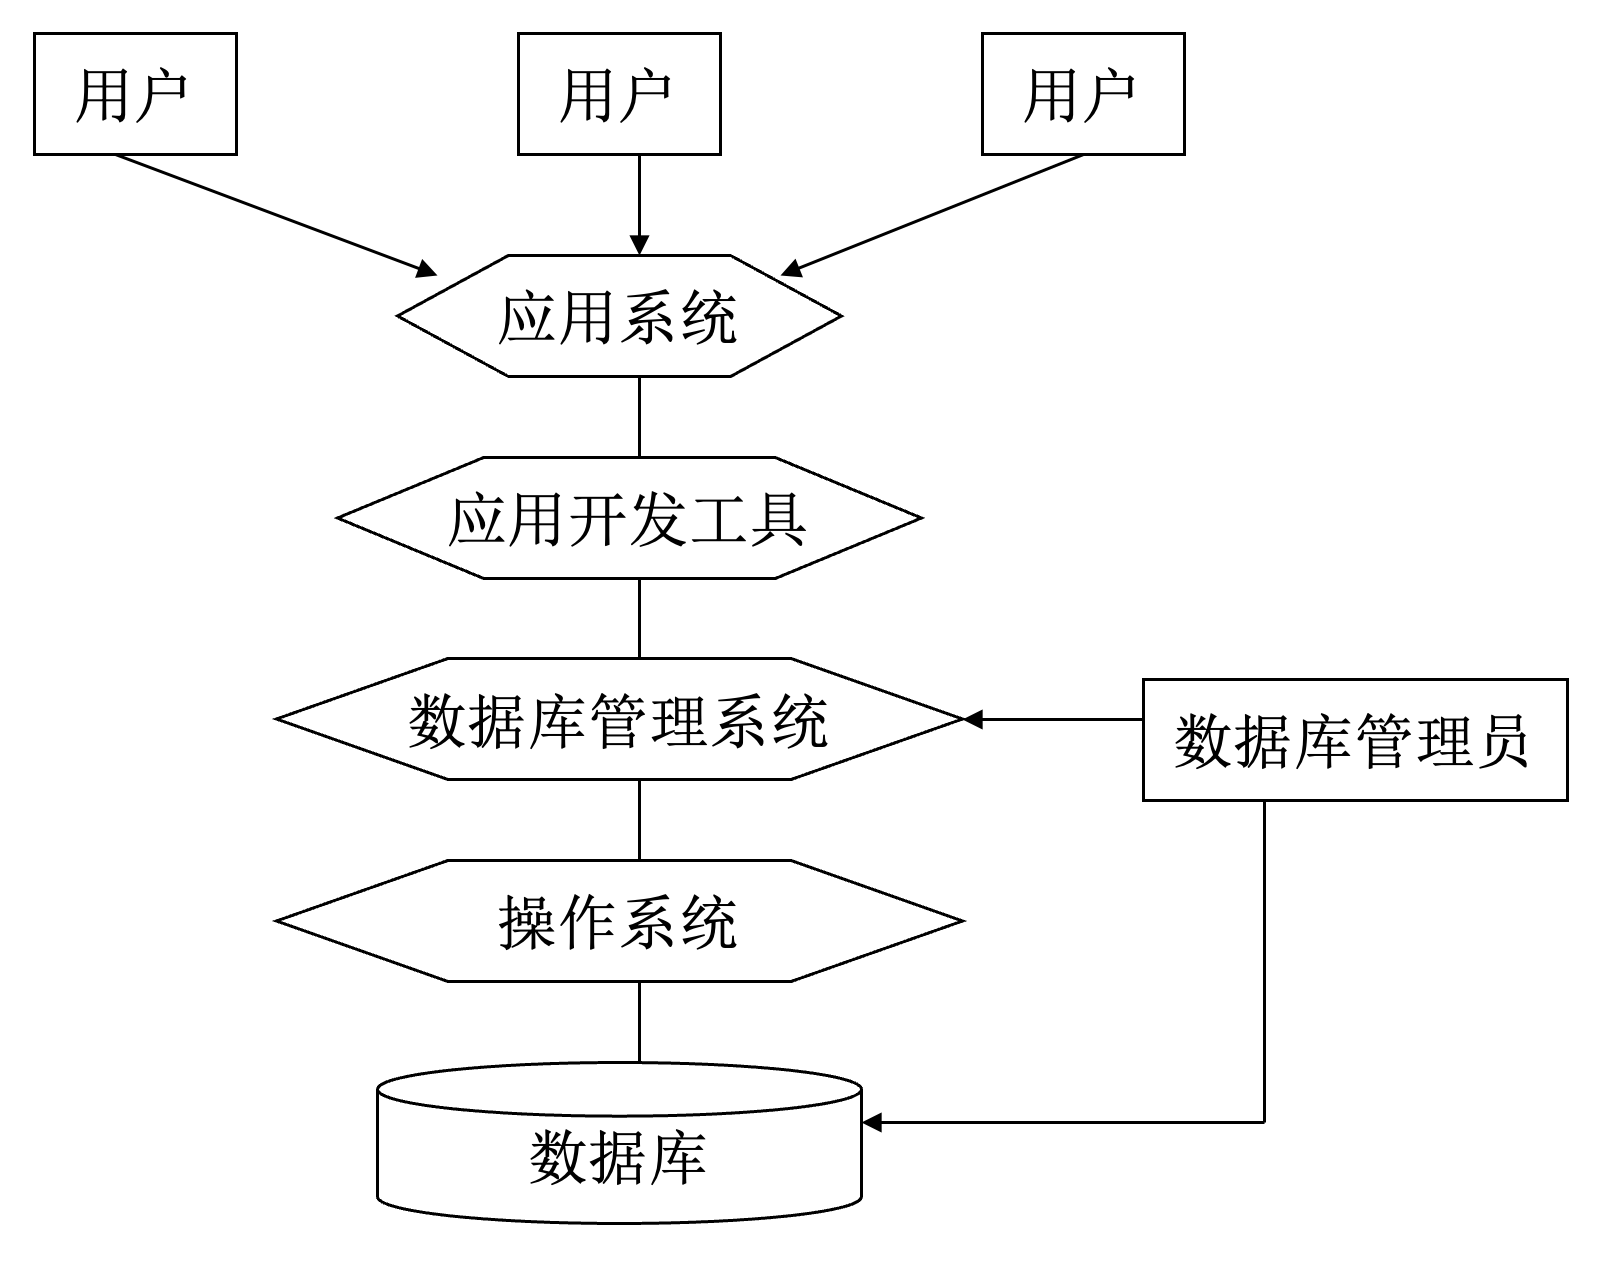
\includegraphics[width=0.45\textwidth]{images/1.1.1.4}
    \vspace{-1em}
\end{figure}

\subsection{数据管理技术的产生和发展}

\vspace{-0.5em}
\begin{longtable}{|W{c}{2.5cm}|W{c}{3.8cm}|W{c}{4.2cm}|m{4cm}<{\centering}|}
    \hline
    \textbf{} & \textbf{人工管理阶段} & \textbf{文件系统阶段} & \textbf{数据库系统阶段}              \\ \hline
    应用背景      & 科学计算            & 科学计算、数据管理       & 大规模数据管理                       \\ \hline
    硬件背景      & 无直接存取存储设备       & 磁盘、磁鼓           & 大容量磁盘、磁盘阵列                    \\ \hline
    软件背景      & 没有操作系统          & 有文件系统           & 有数据库管理系统                      \\ \hline
    处理方式      & 批处理             & 联机实时处理、批处理      & 联机实时处理、分布处理、批处理               \\ \hline
    数据的管理者    & 用户(程序员)         & 文件系统            & 数据库管理系统                       \\ \hline
    数据面向的对象   & 某一应用程序          & 某一应用            & 现实世界                          \\ \hline
    数据的共享程度   & 无共享、冗余度极大       & 共享性差、冗余度大       & 共享性高、冗余度小                     \\ \hline
    数据的独立性    & 不独立、完全依赖于程序     & 独立性差            & 具有高度的物理独立性和一定的逻辑独立性           \\ \hline
    数据的结构化    & 无结构             & 记录内有结构、整体无结构    & 整体结构化,用数据模型描述                 \\ \hline
    数据控制能力    & 应用程序自己控制        & 应用程序自己控制        & 由数据库管理系统提供数据安全性、完整性、并发控制和恢复能力 \\ \hline
    \end{longtable}
\vspace{-1em}

数据库系统的特点:
\begin{itemize}
    \item 数据结构化
    \begin{itemize}
        \item 整体结构化
        \begin{itemize}
            \item 不再仅仅针对某一个应用,而是面向全组织
            \item 不仅数据内部结构化,整体是结构化的,数据之间具有联系
            \item 数据记录可以变长
            \item 数据的最小存取单位是数据项
        \end{itemize}
        \item 数据的用数据模型描述,无需应用程序定义
    \end{itemize}
    \item 数据的共享性高,冗余度低且易扩充
    \begin{itemize}
        \item 数据面向整个系统,可以被多个用户、多个应用共享使用
        \item 数据共享的好处
        \begin{itemize}
            \item 减少数据冗余,节约存储空间
            \item 避免数据之间的不相容性与不一致性 
            \item 使系统易于扩充
        \end{itemize}
    \end{itemize}
    \item 数据独立性高
    \begin{itemize}
        \item 物理独立性
        \begin{itemize}
            \item 指用户的应用程序与数据库中数据的物理存储是相互独立的。当数据的物理存储改变了,应用程序不用改变
        \end{itemize}
        \item 逻辑独立性
        \begin{itemize}
            \item 指用户的应用程序与数据库的逻辑结构是相互独立的。数据的逻辑结构改变了,应用程序不用改变
        \end{itemize}
        \item 数据独立性由数据库管理系统的二级映像功能来保证
        \begin{itemize}
            \item 数据独立性由数据库管理系统的二级映像功能来保证
        \end{itemize}
    \end{itemize}
    \item 数据由数据管理系统统一管理和控制
    \begin{itemize}
        \item 数据库管理系统提供的数据控制功能
        \begin{itemize}
            \item 数据的安全性保护:保护数据以防止不合法的使用造成的数据的泄密和破坏
            \item 数据的完整性检查:保证数据的正确性、有效性和相容性
            \item 并发控制:对多用户的并发操作加以控制和协调,防止相互干扰而得到错误的结果
            \item 数据库恢复:将数据库从错误状态恢复到某一已知的正确状态
        \end{itemize}
    \end{itemize}
\end{itemize}

\section{数据模型}
数据模型是对现实世界数据特征的抽象,用以\textbf{抽象、表示和处理}现实世界中的数据和信息

数据模型应满足三方面要求
\begin{itemize}
    \item 能比较真实地模拟现实世界
    \item 容易为人所理解
    \item 便于在计算机上实现
\end{itemize}

数据模型是数据库系统的核心和基础
\begin{itemize}
    \item 概念模型,也称信息模型
    \begin{itemize}
        \item 按用户的观点来对数据和信息建模,用于数据库设计
    \end{itemize}
    \item 逻辑模型
    \begin{itemize}
        \item 按计算机系统的观点对数据建模,用于DBMS实现
        \item 主要包括网状模型、层次模型、关系模型、面向对象数据模型、对象关系数据模型、半结构化数据模型等
    \end{itemize}
    \item 物理模型
    \begin{itemize}
        \item 是对数据最底层的抽象,描述数据在系统内部的表示方式和存取方法
    \end{itemize}
\end{itemize}

客观对象的抽象过程:两步抽象
\begin{itemize}
    \item 现实世界中的客观对象抽象为概念模型
    \begin{itemize}
        \item 将现实世界抽象为信息世界
    \end{itemize}
    \item 把概念模型转换为特定DBMS支持的数据模型
    \begin{itemize}
        \item 将信息世界转换为机器世界
    \end{itemize}
\end{itemize}

\begin{figure}[H]
    \vspace{-0.5em}
	\centering
	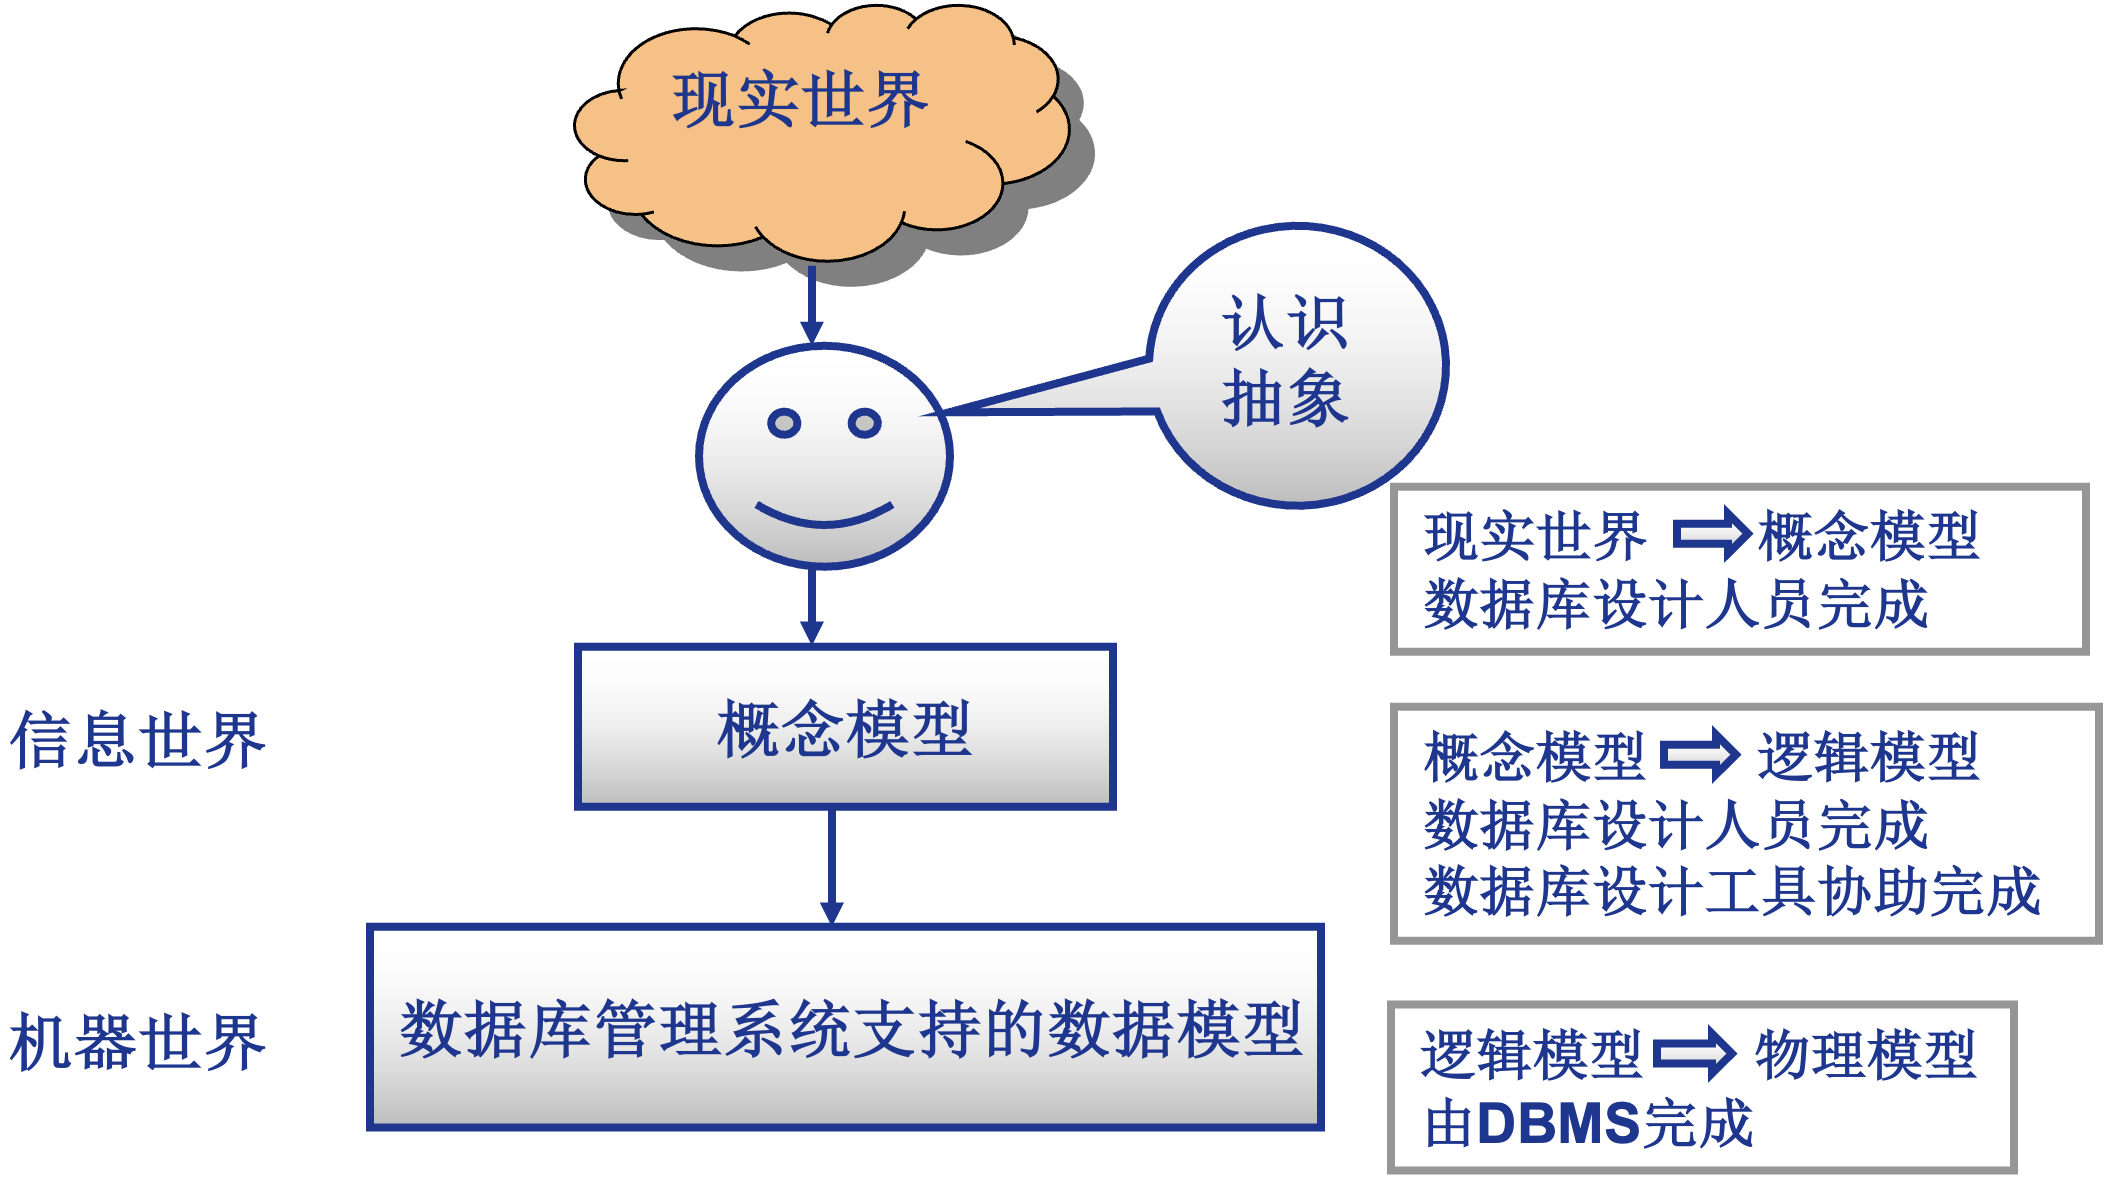
\includegraphics[width=0.65\textwidth]{images/1.2}
    \vspace{-1em}
\end{figure}

数据模型的组成要素
\begin{itemize}
    \item 数据结构:描述数据库的组成对象,以及对象之间的联系
    \begin{itemize}
        \item 描述的内容
        \begin{itemize}
            \item 与对象的类型、内容、性质有关
            \item 与数据之间联系有关
        \end{itemize}
        \item 数据结构是对系统静态特性的描述
    \end{itemize}
    \item 数据操作:对数据库中各种对象(型)的实例(值)允许执行的操作的集合,包括操作及有关的操作规则
    \begin{itemize}
        \item 数据操作的类型
        \vspace{-0.8em}
	    \begin{multicols}{2}
        \begin{itemize}
            \item 查询
            \item 更新(包括插入、删除、修改)
        \end{itemize}
	    \end{multicols}
	    \vspace{-1em}
        \item 数据模型对操作的定义
        \begin{itemize}
            \item 操作的确切含义、操作符号、操作规则(如优先级)
            \item 实现操作的语言
        \end{itemize}
    \end{itemize}
    \item 数据的完整性约束条件:一组完整性规则的集合
    \begin{itemize}
        \item 完整性规则:给定的数据模型中数据及其联系所具有的制约和依存规则
        \item 用以限定符合数据模型的数据库状态以及状态的变化,以保证数据的正确、有效和相容
        \item 数据模型对完整性约束条件的定义
        \begin{itemize}
            \item 反映和规定必须遵守的基本的通用的完整性约束条件
            \item 提供定义完整性约束条件的机制,以反映具体应用所涉及的数据必须遵守的特定的语义约束条件
        \end{itemize}
    \end{itemize}
\end{itemize}

\section{数据库系统的结构}

\subsection{数据库系统模式的概念}
\begin{itemize}
    \item 在数据库模型中有“型“和”值“的概念
    \begin{itemize}
        \item 型是指对某一类数据的结构和属性的说明
        \item 值是型的一个具体赋值
    \end{itemize}
    \item 模式是数据库中全体数据的逻辑结构和特征的描述,仅仅涉及型的描述,不涉及具体值
    \item 模式的一个具体的值称为模式的实例,同一个模式可以有多个实例
\end{itemize}

\subsection{数据库的三级模式结构}
\begin{figure}[H]
    \vspace{-0.5em}
	\centering
	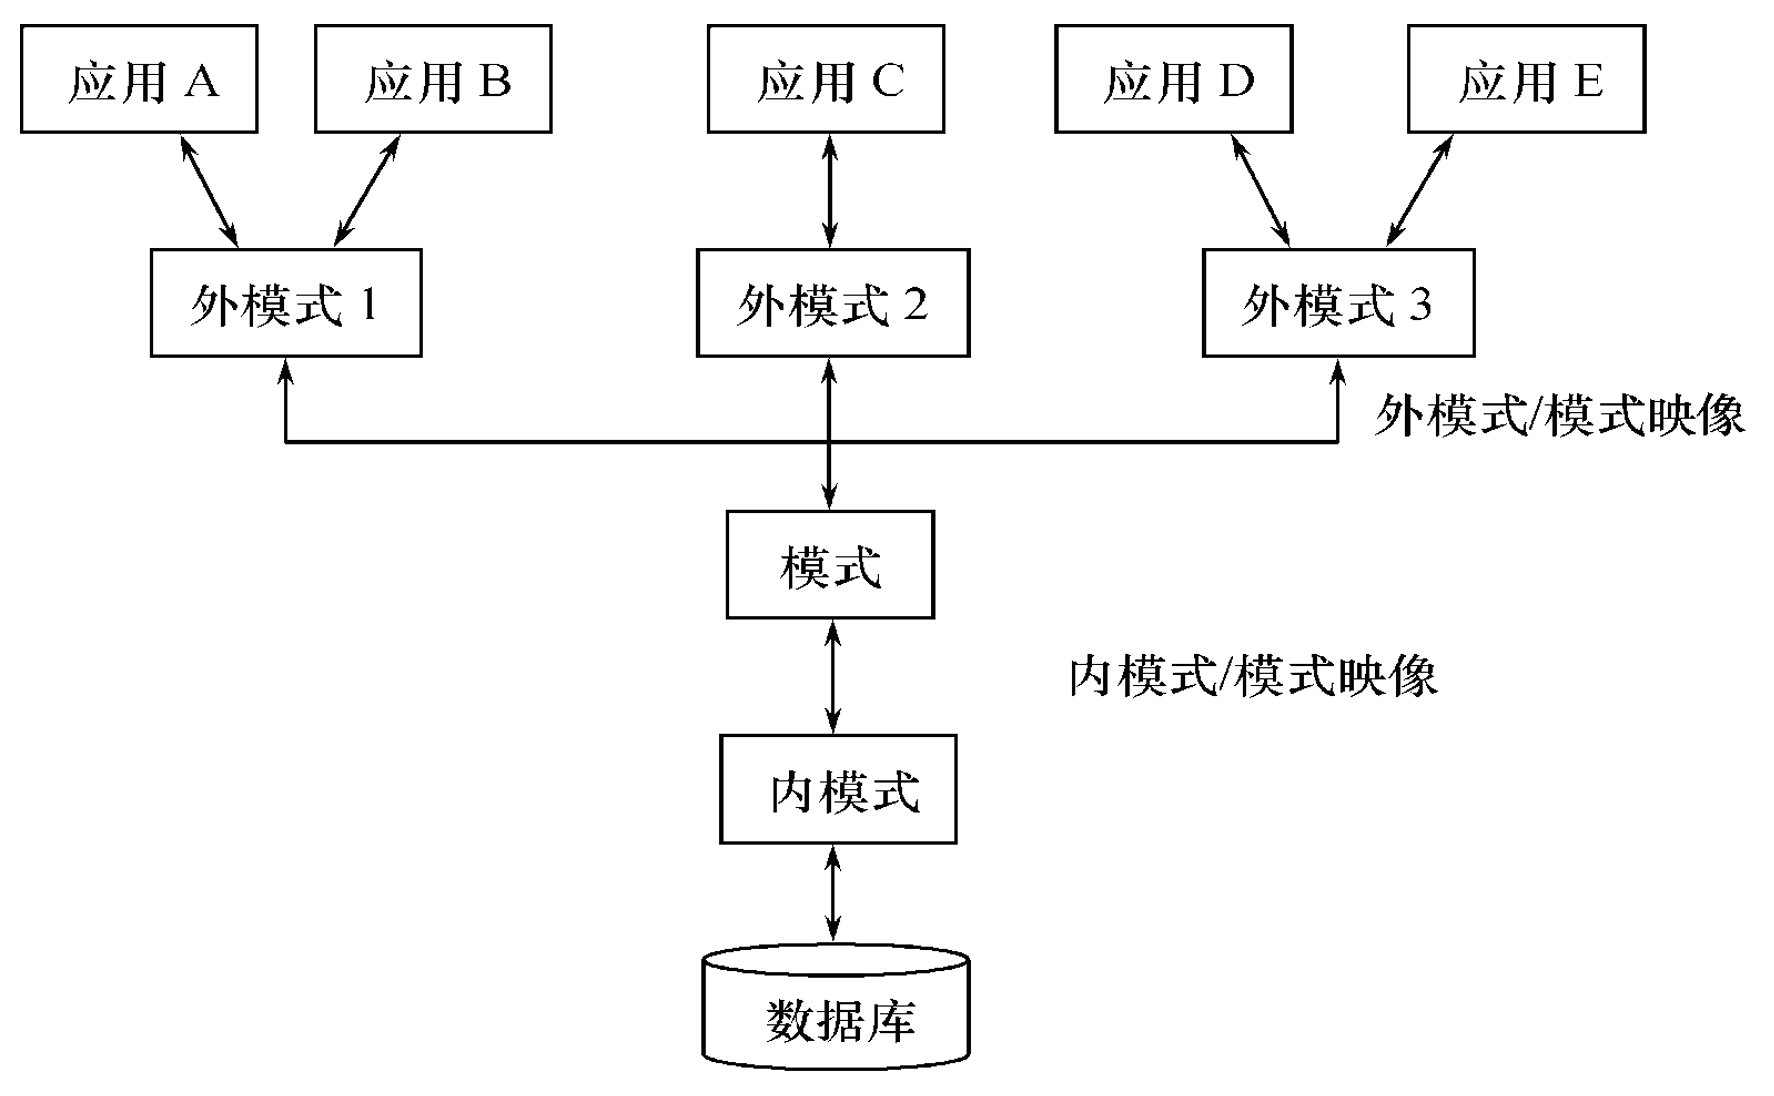
\includegraphics[width=0.65\textwidth]{images/1.3.2}
    \vspace{-1em}
\end{figure}

\subsubsection{模式}
\begin{itemize}
    \item 模式,也称逻辑模式,是数据库中全体数据的逻辑结构和特征的描述,是所有用户的公共数据视图
    \item 一个数据库只有一个模式
    \item 模式是数据库系统模式结构的中间层,与数据的物理存储细节和硬件环境无关,与具体的应用程序、开发工具及高级程序设计语言无关
    \item 定义模式时不仅要定义数据的逻辑结构,而且要定义数据之间的联系,定义数据有关的安全性、完整性要求
\end{itemize}

\subsubsection{外模式}
\begin{itemize}
    \item 外模式也称子模式或用户模式,它是数据库用户(包括应用程序员和最终用户)使用的局部数据的逻辑结构和特征的描述,是数据库用户的数据视图,是与某一应用有关的数据的逻辑表示
    \item 模式与外模式的关系:一对多
    \begin{itemize}
        \item 外模式通常是模式的子集
        \item 一个数据库可以有多个外模式。反映了不同的用户的应用需求、看待数据的方式、对数据保密的要求
        \item 对模式中同一数据,在外模式中的结构、类型、长度、保密级别等都可以不同
    \end{itemize}
    \item 外模式与应用的关系:一对多
    \begin{itemize}
        \item 同一外模式也可以为某一用户的多个应用系统所使用
        \item 但一个应用程序只能使用一个外模式
    \end{itemize}
    \item 外模式的用途
    \begin{itemize}
        \item 保证数据库安全性的一个有力措施
        \item 每个用户只能看见和访问所对应的外模式中的数据
    \end{itemize}
\end{itemize}

\subsubsection{内模式}
内模式也称存储模式,是数据物理结构和存储方式的描述,是数据在数据库内部的表示方式。一个数据库只有一个内模式。
\vspace{-0.8em}
\begin{multicols}{2}
    \begin{itemize}
        \item 记录的存储方式
        \item 索引的组织方式
        \item 数据是否压缩存储
        \item 数据是否加密
        \item 数据存储记录结构的规定
    \end{itemize}
\end{multicols}
\vspace{-1em}

\subsection{数据库的二级映像功能与数据独立性}
数据库系统的三级模式是数据的三个抽象级别,它把数据的具体组织留给数据库管理系统,使用户能逻辑地、抽象地处理数据,而不必关心数据在计算机中的具体表示方式与存储方式

为了能够在系统内部实现这三个抽象层次的联系和转换,数据库管理系统在这三级模式之间提供了两层映像:外模式/模式映像和模式/内模式映像

\subsubsection{外模式/模式映像}
\begin{itemize}
    \item 模式描述的是数据的全局逻辑结构
    \item 外模式:描述的是数据的局部逻辑结构 
    \item 同一个模式可以有任意多个外模式 
    \item 每一个外模式,数据库系统都有一个外模式/模式映象,定义外模式与模式之间的对应关系
    \item 映象定义通常包含在各自外模式的描述中
    \item 保证数据的逻辑独立性
    \begin{itemize}
        \item 当模式改变时,数据库管理员对外模式/模式映象作相应改变,使外模式保持不变
        \item 应用程序是依据数据的外模式编写的,应用程序不必修改,保证了数据与程序的逻辑独立性,简称数据的逻辑独立性
    \end{itemize}
\end{itemize}

\subsubsection{模式/内模式映像}
\begin{itemize}
    \item 模式/内模式映象定义了数据全局逻辑结构与存储结构之间的对应关系。
    \item 数据库中模式/内模式映象是唯一的
    \item 该映象定义通常包含在模式描述中
    \item 保证数据的物理独立性
    \begin{itemize}
        \item 当数据库的存储结构改变了(例如选用了另一种存储结构),数据库管理员修改模式/内模式映象,使模式保持不变
        \item 应用程序不受影响。保证了数据与程序的物理独立性,简称数据的物理独立性
    \end{itemize}
\end{itemize}

\subsubsection{数据库的二级映像}
\begin{itemize}
    \item 数据库模式
    \begin{itemize}
        \item 即全局逻辑结构是数据库的中心与关键
        \item 独立于数据库的其他层次 
        \item 设计数据库模式结构时应首先确定数据库的逻辑模式
    \end{itemize}
    \item 数据库的内模式
    \begin{itemize}
        \item 依赖于它的全局逻辑结构
        \item 独立于数据库的用户视图,即外模式
        \item 独立于具体的存储设备 
        \item 将全局逻辑结构中所定义的数据结构及其联系按照一定的物理存储策略进行组织,以达到较好的时间与空间效率
    \end{itemize}
    \item 数据库的外模式
    \begin{itemize}
        \item 面向具体的应用程序
        \item 定义在逻辑模式之上
        \item 独立于存储模式和存储设备
        \item 当应用需求发生较大变化,相应外模式不能满足其视图要求时,该外模式就得做相应改动
        \item 设计外模式时应充分考虑到应用的扩充性
    \end{itemize}
    \item 特定的应用程序
    \begin{itemize}
        \item 在外模式描述的数据结构上编制的
        \item 依赖于特定的外模式
        \item 与数据库的模式和存储结构独立
        \item 不同的应用程序有时可以共用同一个外模式
    \end{itemize}
    \item 数据库的二级映像
    \begin{itemize}
        \item 保证了数据库外模式的稳定性
        \item 从底层保证了应用程序的稳定性,除非应用需求本身发生变化,否则应用程序一般不需要修改
    \end{itemize}
    \item 数据与程序之间的独立性,使得数据的定义和描述可以从应用程序中分离出去
    \item 数据的存取由数据库管理系统管理
    \begin{itemize}
        \item 简化了应用程序的编制
        \item 大大减少了应用程序的维护和修改
    \end{itemize}
\end{itemize}

\section{数据库系统的组成}

\subsection{硬件平台及数据库}
数据库系统对硬件资源的要求
\begin{itemize}
    \item 足够大的内存
    \item 足够的大的磁盘或磁盘阵列等设备
    \item 较高的通道能力,提高数据传送率
\end{itemize}

\subsection{软件}
数据库系统的软件主要包括
\begin{itemize}
    \item 数据库管理系统
    \item 支持数据库管理系统运行的操作系统
    \item 与数据库接口的高级语言及其编译系统
    \item 以数据库管理系统为核心的应用开发工具
    \item 为特定应用环境开发的数据库应用系统
\end{itemize}

\subsection{人员}
\begin{figure}[H]
    \vspace{-0.5em}
	\centering
	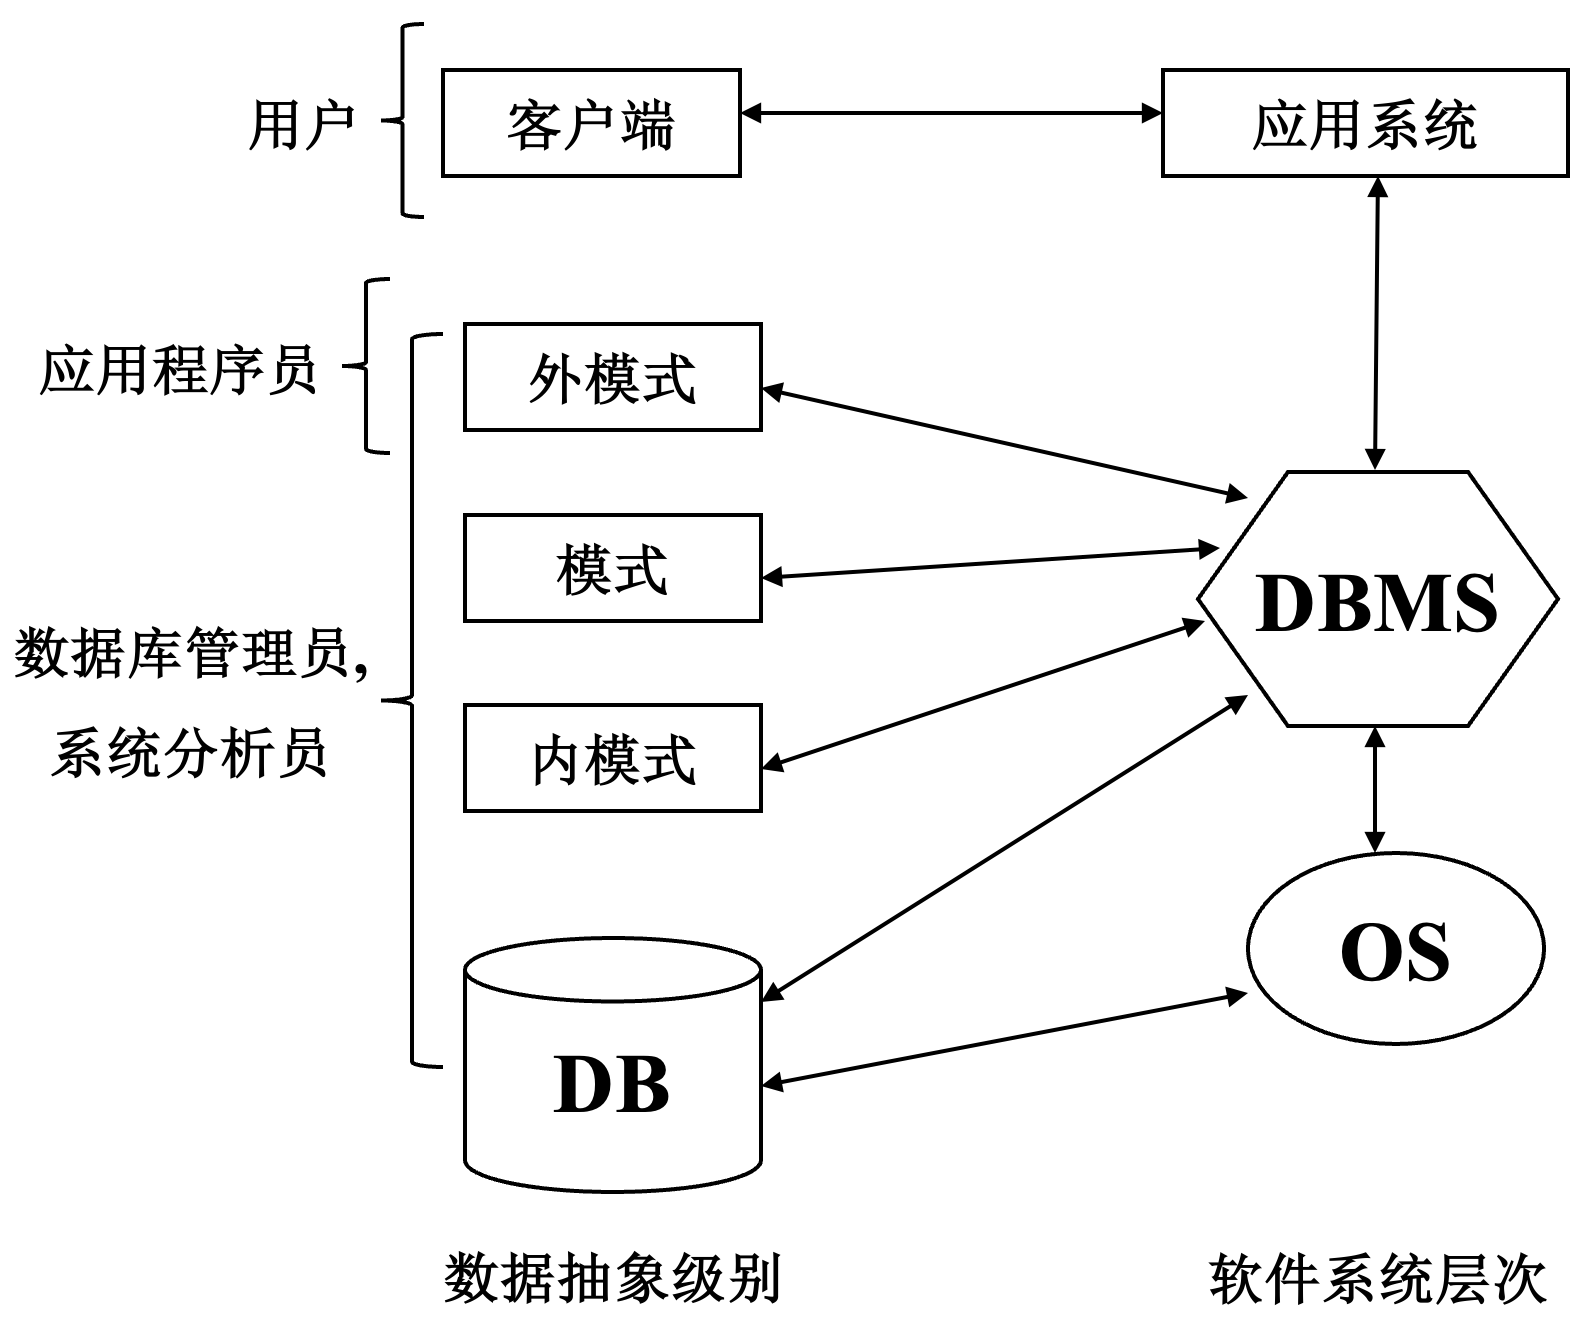
\includegraphics[width=0.5\textwidth]{images/1.4.3}
    \vspace{-1em}
\end{figure}

数据库管理人员
\begin{itemize}
    \item 决定数据库中的信息内容和结构
    \item 决定数据库的存储结构和存取策略
    \item 定义数据的安全性要求和完整性约束条件
    \item 监控数据库的使用和运行:周期性转储数据库
    \vspace{-0.8em}
    \begin{multicols}{2}
        \begin{itemize}
            \item 数据文件
            \item 日志文件
            \item 系统故障恢复
            \item 介质故障恢复
            \item 监视审计文件
        \end{itemize}
    \end{multicols}
    \vspace{-1em}
    \item 数据库的改进和重组
    \begin{itemize}
        \item 性能监控和调优
        \item 定期对数据库进行重组织,以提高系统的性能
        \item 需求增加和改变时,数据库须需要重构造
    \end{itemize}
\end{itemize}

系统分析员
\begin{itemize}
    \item 负责应用系统的需求分析和规范说明
    \item 与用户及数据库管理员结合,确定系统的硬软件配置
    \item 参与数据库系统的概要设计
\end{itemize}

数据库设计人员
\vspace{-0.8em}
\begin{multicols}{2}
    \begin{itemize}
        \item 参加用户需求调查和系统分析
        \item 确定数据库中的数据
        \item 设计数据库各级模式
    \end{itemize}
\end{multicols}
\vspace{-1em}


应用程序员
\vspace{-0.8em}
\begin{multicols}{2}
    \begin{itemize}
        \item 设计和编写应用系统的程序模块
        \item 进行调试和安装
    \end{itemize}
\end{multicols}
\vspace{-1em}


最终用户:最终用户通过应用系统的用户接口使用数据库
\begin{itemize}
    \item 偶然用户
    \begin{itemize}
        \item 不经常访问数据库,但每次访问数据库时往往需要不同的数据库信息 
        \item 企业或组织机构的高中级管理人员
    \end{itemize}
    \item 简单用户
    \begin{itemize}
        \item 主要工作是查询和更新数据库
        \item 银行的职员、机票预定人员、旅馆总台服务员
    \end{itemize}
    \item 复杂用户
    \begin{itemize}
        \item 工程师、科学家、经济学家、科技工作者等
        \item 直接使用数据库语言访问数据库,甚至能够基于数据库管理系统的应用程序接口编制自己的应用程序
    \end{itemize}
\end{itemize}

